% Methods
In this chapter, a description of event selection is given, as well as definitions of
key physical variables and how they are used to select events. Then, a procedure regarding
how the signal sample is manipulated to produce a high statistics off-shell Higgs sample is presented.
Finally, the binning of variables used to obtain the results is determined and defined.

\section{Event selection and physical variables}
Proton bunches cross each at a rate of about \SI{400}{\mega\hertz} in the beam line of
the LHC, naturally, not all of these crossings are recorded due to both technical
limitation of the electronics as well as the fact that the vast majority of these
crossings don't produce inelastic collision that is energetic enough to be interesting.

After the selection of Level 1 (L1) trigger and the higher level trigger (HLT), less than 1000
events per second are permanently recorded and would go to off-line, full reconstruction. Among these,
we only select the ones that passes certain HLT trigger, for 2018 data set:
\begin{itemize}
    \item HLT\_Mu17\_TrkIsoVVL\_Mu8\_TrkIsoVVL\_DZ\_Mass3p8
    \item HLT\_IsoMu24
    \item HLT\_Ele23\_Ele12\_CaloIdL\_TrackIdL\_IsoVL
    \item HLT\_DoubleEle25\_CaloIdL\_MW
    \item HLT\_DoublePhoton70
    \item HLT\_Ele32\_WPTight\_Gsf
    \item HLT\_Photon200
\end{itemize}
Most of the trigger names are self-explanatory, for example, the numbers are the momentum 
threshold (in \si{\giga\electronvolt}) to trigger them. The HLT is the starting point of the analysis. The
purpose of the triggers is to ensure the events in the corresponding samples would contain the physics
we wanted (since run data samples are divided according to what triggers they passed).

The next step is to `add' composite variables that is significant to the physics of interests as
well as making base-line cuts on the events.
The jets are all AK4 jets unless mentioned otherwise, and a special type of jets, called b-tagged
jets are \cc{produced} identified using the DeepFlavour algorithm.\cite{deepflavour} \add{These are jets
likely originated from relatively long-lived bottom quarks judging from a combination of many measurements 
including the displacement of verteces.} 
We shall also define a few of the
uncommon variables in the list, and physical motivations are given in the following
paragraphs.

After mandating passage of the set of triggers above, based on more delicate physics reasons, 
the baseline cuts are:
\begin{itemize}
    \item $\met > 125 \gev$:
        the signal process creates true $\met$ with neutrinos, this cut also reduce bkg such
        as DY.
    \item Both leptons have $p_\mathrm{T} > \SI{25}{\giga\electronvolt}$
    \item $\abs{\Delta\phi_{\ell\ell\_\met}} > 1.0$
    \item $\abs{\Delta\phi_{\ell\ell\mathrm{Jets}\_\met}} > 2.5$
    \item $\abs{m_{\ell\ell} - \SI{91.2}{\giga\electronvolt}} < \SI{15}{\giga\electronvolt}$:
        the signal process consists of $\mathrm{Z}\rightarrow{}\ell\ell$, we
        require the di-lepton system has a mass that is consistent within the Z mass peak.
    \item $p_\mathrm{T}^{\ell\ell} > \SI{55}{\giga\electronvolt} $: 
        the Drell–Yan (DY) process creates a lot of backgrounds events, but their di-leptons
        go back-to-back with expected value of this variable close to 0.
    \item No ak4-jet b-tagged jet ($\Delta{}R=0.4$, loose b-tagging working point (WP))
    \item $\min{\abs{ \Delta\phi_{\mathrm{j}\_\met}}} > 0.25$
\end{itemize}
In addition, to reduce the detector effects at high pseudo rapidity angels:
\begin{itemize}
    \item $\eta_\mu< 2.4$
    \item $\eta_e< 2.5$
\end{itemize}

First and most importantly, the $\met$ cut reduces background from DY significantly since they don't havd
real $\met$.  Notice many of the 
cuts are related to angles between various physical objects presented in the
reconstruction. The reason is simple: the signal events, where Higgs goes to ZZ and one Z
goes to 2 charged leptons and the other goes to 2 neutrinos, ideally would have the two Z's 
`back-to-back' in Higgs boson's rest frame, leading to a large angel in the transverse plane.
% ( assuming the $\met$ mainly comes from the two neutrinos, of course)

Furthermore, in background events which do not contain this kinematic feature, the
correlation in the directions of $\vec{E}_{T}^\mathrm{missing}$ and the transverse momentum of the leptons is weaker.

To use this kinematic feature to increase signal to background ratio, we define 
$\abs{\Delta\phi_{\ell\ell\_\met}}$ as the azimuthal angel (perpendicular to 
the beam line) between the di-lepton system and the transverse missing energy. In the
signal events that produce 0 jet, this variable should be $\pi$. The cut is lowered to $1.0$ 
due to the finding that in the (not so rare) cases where there are jet(s) recoiling against
the ZZ system, this variable can go quite low.

This leads to the next variable on the list, $\abs{\Delta\phi_{\ell\ell\mathrm{Jets}\_\met}}$, which
is almost the same except that we add all jets' momentum into the di-lepton system to account
for the events that have produced jets, which in turn would cause the angel be lower in
a multi-body final state.

\add{Also, a veto on the b-tagged jet is placed to reduce the background events originated from a pair
of top quarts ($t\bar{t}$) since top quark always decays to a bottom quark.} 

Finally, $\min{\abs{ \Delta\phi_{\mathrm{j}\_\met}}}$ is the minimum azimuthal angel difference between
any of the jet (that passes cuts) and the $\met$, it exist because jets are one of the 
most difficult physical objects measure, they often create so-called instrumental $\met$ due to jet
mis-measurements and it can be quite large in magnitude. However, such mis-measurements often yield large
$\met$ in the direction of the original jet. This cuts requires angular separation since in signal process,
the jet recoils against ZZ system.

We also define variables that are not cut on, but are used for fitting:
\be
D_{j j}^{V B F}=\frac{P_{S M}^{V B F}(\vec{\Omega})}{P_{S M}^{g g}(\vec{\Omega})+P_{S M}^{V B F}(\vec{\Omega})}
\ee
as first introduced in another CMS paper~\cite{djjvbf}. In short, this variable (discriminator) is sensitive
to the VBF physics and the correlation between (angels and mass of) the outgoing jets resulted from the
VBF topology. At the same time:
\be
\mtzz={\left[\sqrt{p_{\mathrm{T}, \ell\ell}^2+m_{2 \ell}^2}+\sqrt{E_{\mathrm{T}}^{\mathrm{miss}^2}+m_\mathrm{Z}^2}\right]}^2-\left[\vec{p}_{\ell\ell}+\vec{E}_{\mathrm{T}}^{\mathrm{miss}}\right]^{2}
\ee
is defined based on the hypothesis that the $\met$ is comprised of mainly the two neutrinos
from one of the Z bosons. We shall see the usefulness of this variable in channels where
not enough jets are present to construct the $D_{j j}^{V B F}$ variable.

On top of the cuts stated in the beginning, several $\met$ filters exist to remove detector 
anomolies. Lepton isolated tracks veto is implemented
in the underlying analysis framework to \cc{reject events with pathological reconstruction.}
\add{remove events with additional leptons that are likely backgrounds, such as those can be found in WZ.}
% \missingfigure{Show how much backgrounds are gone for maybe 2 samples}

\section{Signal samples re-weighting}
\label{sec:sig_rewgt}
% \begin{itemize}
%     \item Physics of Higgs signal sample (the weight, ME)
%     \item the need for pieceing together samples with different LHE Mass
%     \item results (also see appendix A)
% \end{itemize}
Extra attention was given to the off-shell Higgs sample used in this thesis and two different kinds
of re-weighting of the simulated events are applied in to produced a MC sample with wide
mass spectrum way beyond the mass of Higgs ($\approx \SI{125}{\giga\electronvolt}$). We use the
gluon fusion Higgs (ggH) sample to illustrate the procedures, the same procedures are applied to
the VBF samples as well.

We start by generating separate samples with different Higgs mass (LHECandMass).
This is the mass of Higgs terms appears in the propagator on 
the R.H.S of Eq.~\ref{eqn:diff_xsec} as mentioned before. The raw distribution of the true mass
in different samples (without any weight) is shown in Fig.~\ref{fig:LHE_raw} (left). As expected, 
the peak of the distribution moves to the right as the mass of the sample becomes larger, at the
same time, the `peak' of samples with very large mass are wider because the width of the Higgs increases.
We also see that for some lower mass
samples (200, 300, 400 etc.), they have a cut-off (due to insufficnet statistics) beyond $\mathrm{M}\approx2500$ which means they have 0
statistics beyond that mass range. After applying the GEN, PU, and ME weights given by their
individual MC process and JHUGen MELA, as shown in Fig.~\ref{fig:LHE_raw},
we see that they are consistent with each others' line shape. However, it is clear
that:
\begin{enumerate}[label=(\roman*)]
    \item Lower mass samples have insufficnet statistics in the tail region
    \item Samples have poor statistics in mass windows that are 
        far from their true mass (as listed in the legend).
\end{enumerate}
The second point is best illustrated by the wide spikes of lower mass samples near their `cut-offs',
as well as the visible fluctuations of high-mass samples in the mass region (don't let the 
visual mislead you, the plots are in semi-log scale).
\begin{figure}[htb]
    \begin{center}
        \subfloat[]{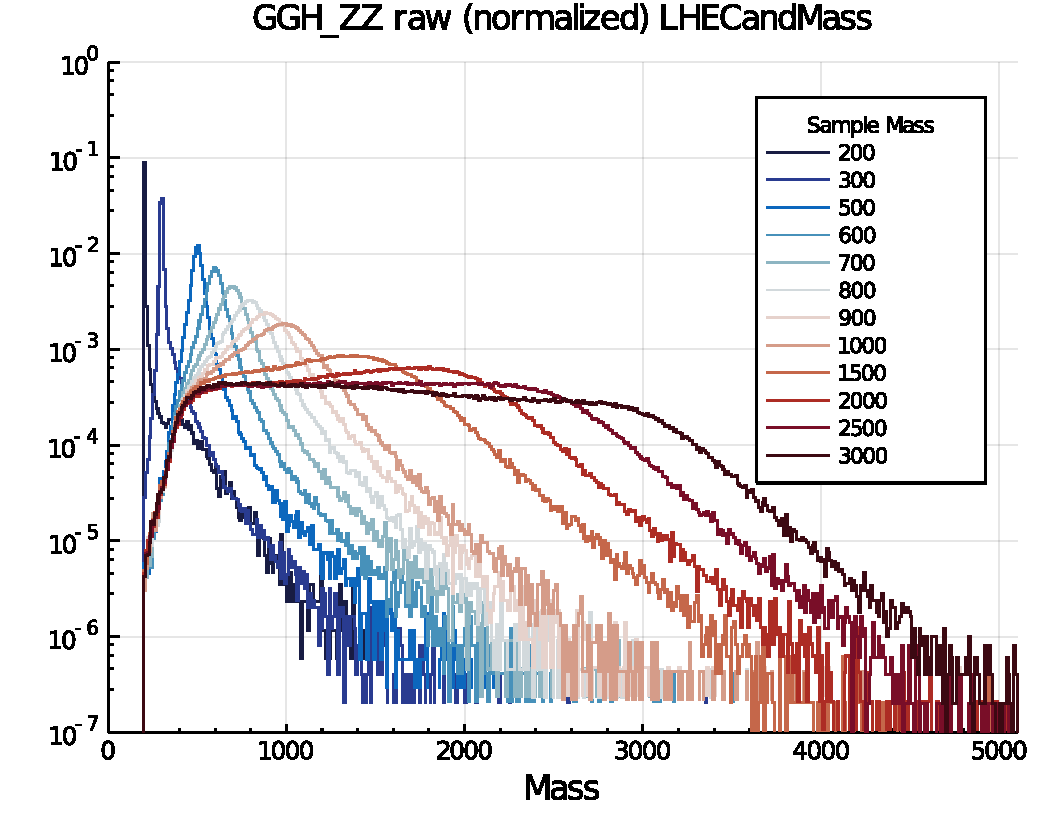
\includegraphics[width=.5\linewidth]{fig/LHE_Raw.pdf}}
        \subfloat[]{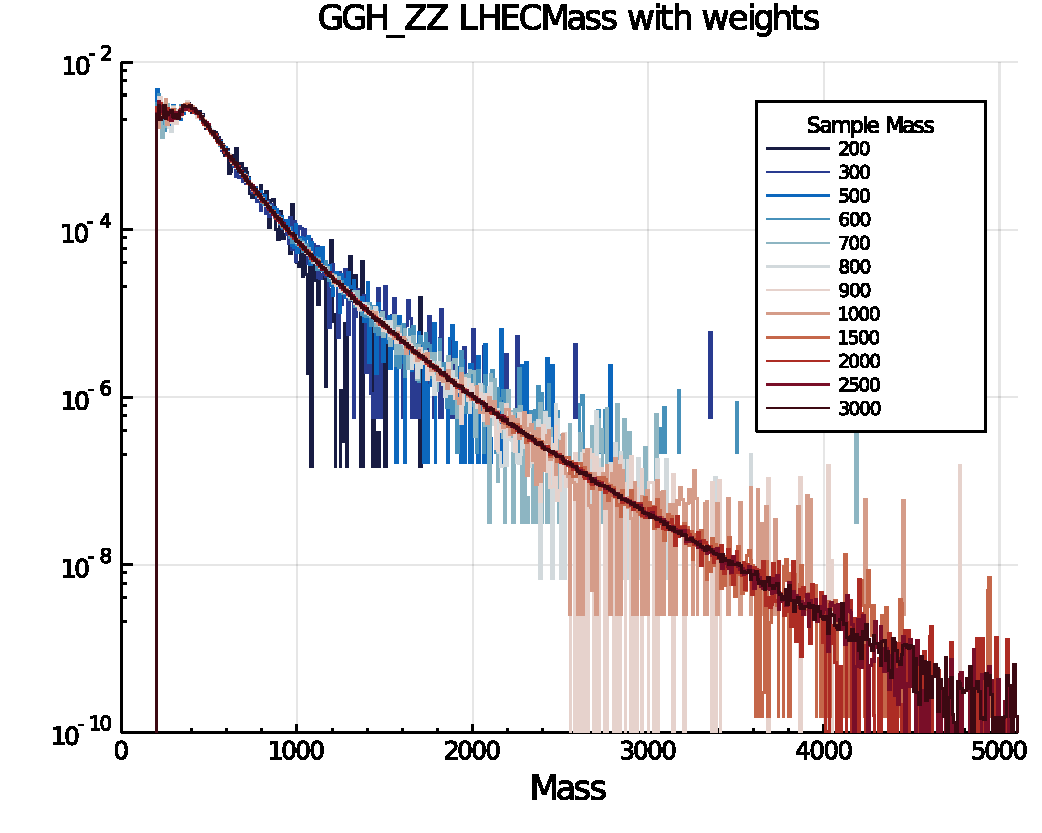
\includegraphics[width=.5\linewidth]{fig/LHE_PUME_wgts.pdf}}\\
    \end{center}
    \caption{Unit normalized distributions of LHECandMass before (left) and after (right) applying
        the weights. Together they show a need to combine samples for a wide-range, high
    statistics signal sample. Bin size = \SI{10}{\giga\electronvolt}.}
    \label{fig:LHE_raw}
\end{figure}

The goal of the combination of samples is to use all the events, but with a correction weight
such that each sample has a higher weight in the region where they poses good statistics
while keeping the overall normalization stays unchanged. To do this, we pick a list of
`mass windows' with edges sitting on the true masses of the samples, and we define effective
number of events $\mathrm{N}_\mathrm{eff} = \frac{(\sum\mathrm{wgts})^2}{\sum(\mathrm{wgts}^2)}$
within each mass window. Here, the wgts corresponds to the product of PU wgt, GEN wgt, K-factor, and ME weight for
the GGH sample in consideration. For a specific GGH sample $i_0$ and its events fall in a mass 
window $j$, $\mathrm{N}_\mathrm{eff}^{i_0j}$ is first obtained and a re-weighting factor can be computed:
\be
\mathrm{wgt}_\mathrm{window}^{i_0j} = 
\frac{\mathrm{N}_\mathrm{eff}^{i_0j}}{\sum_i\mathrm{N}_\mathrm{eff}^{ij}}
\ee
This factor is applied to all events from sample $i_0$ within the window $j$. Conceptually,
the effective number of events ensures the weight is not skewed by the difference in the overall
normalization of samples, and in each of the mass windows, samples with more concentrated
statistics in that window are given a higher weight. In Fig.~\ref{fig:window_wgt_matrix} (a), a
clear diagonal pattern can be seen, physically it means that samples with higher true 
mass are given a higher weight in tail mass windows--- consistent with the expected outcome. Complete
table of weights can be founed in Appendix~\ref{apdx:window_wgts}.
\begin{figure}[htb]
    \begin{center}
        \subfloat[]{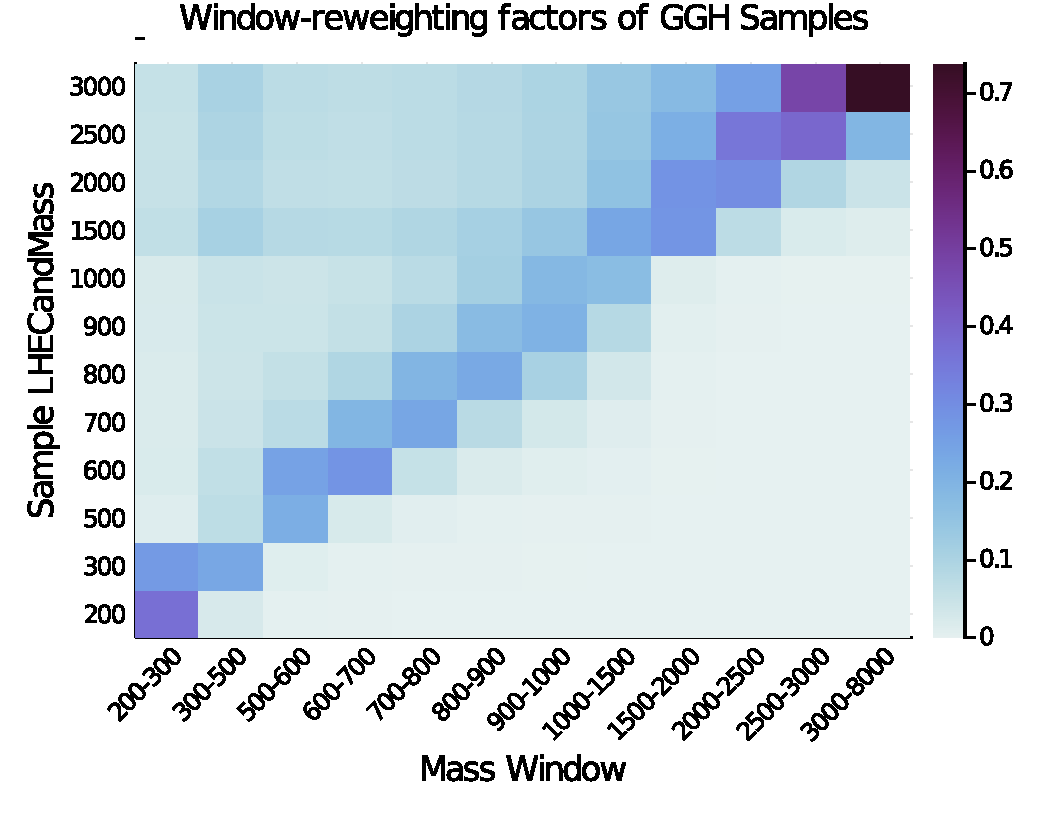
\includegraphics[width=.5\linewidth]{fig/Window_wgt_GGH.pdf}}
        \subfloat[]{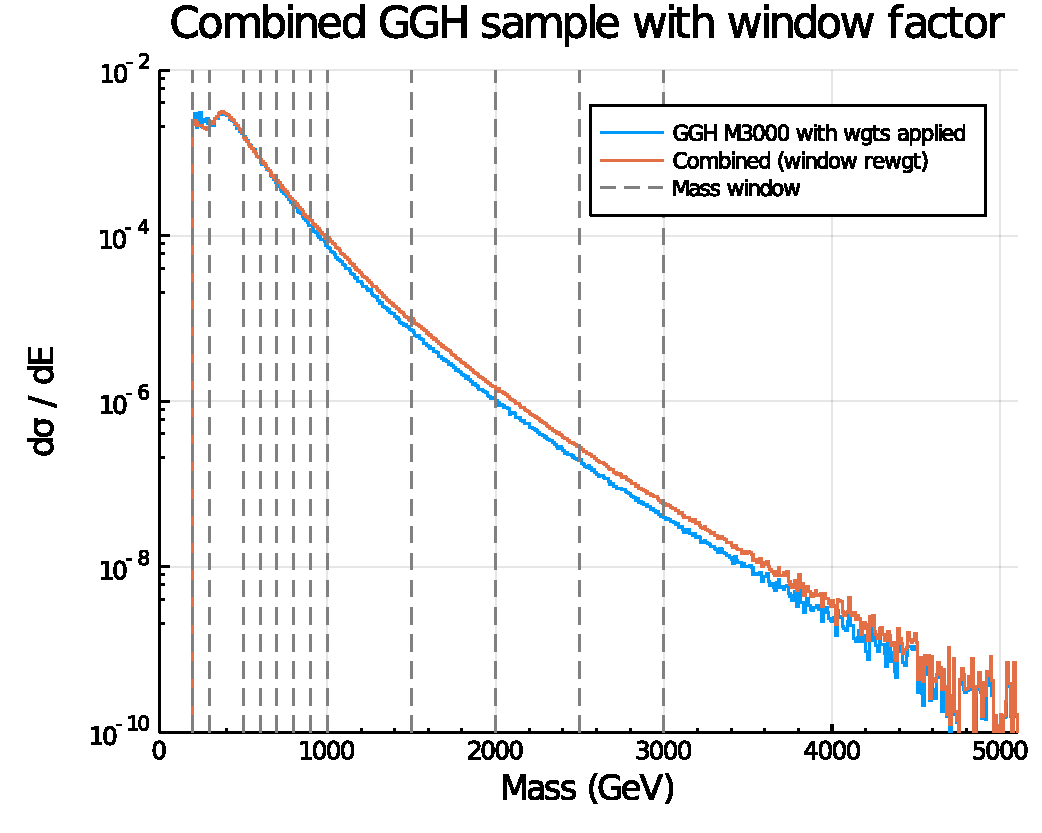
\includegraphics[width=.5\linewidth]{fig/LHC_compare_windowwgt.pdf}}
    \end{center}
    \caption{Heatmap of window re-weight factors of different samples and mass windows (left);
    effects of applying window factors for the combined sample(right)}
    \label{fig:window_wgt_matrix}
\end{figure}

However, even with the unit normalization, there are still inconsistency in the shape as shown
in Fig.~\ref{fig:window_wgt_matrix} (b). This is likely because the finite number of events
and non-infinitesimal mass window size used. We introduce another correction factor for
this small artifacts. Iteratively going through every sample, between the previous and the
next one, derive a sample mass factor based on:
\be
\mathrm{wgt}_\mathrm{mass}^{i, i+1} = \frac{\sum{\mathrm{wgt}_\mathrm{i}}}{\sum{\mathrm{wgt}_\mathrm{i+1}}}
\text{, for events that has Mass between sample mass of $i$ and $i+1$}
\ee

\begin{figure}[htb]
    \begin{center}
        \subfloat[]{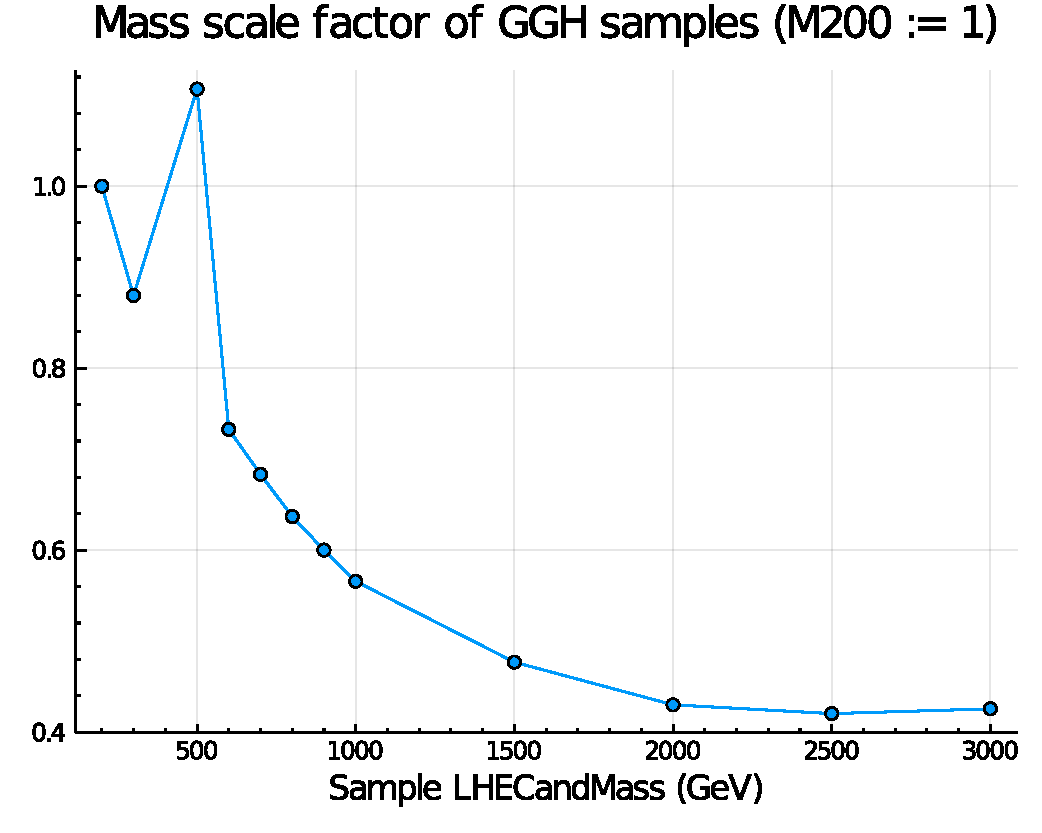
\includegraphics[width=.5\linewidth]{fig/Mass_wgt_GGH.pdf}}
        \subfloat[]{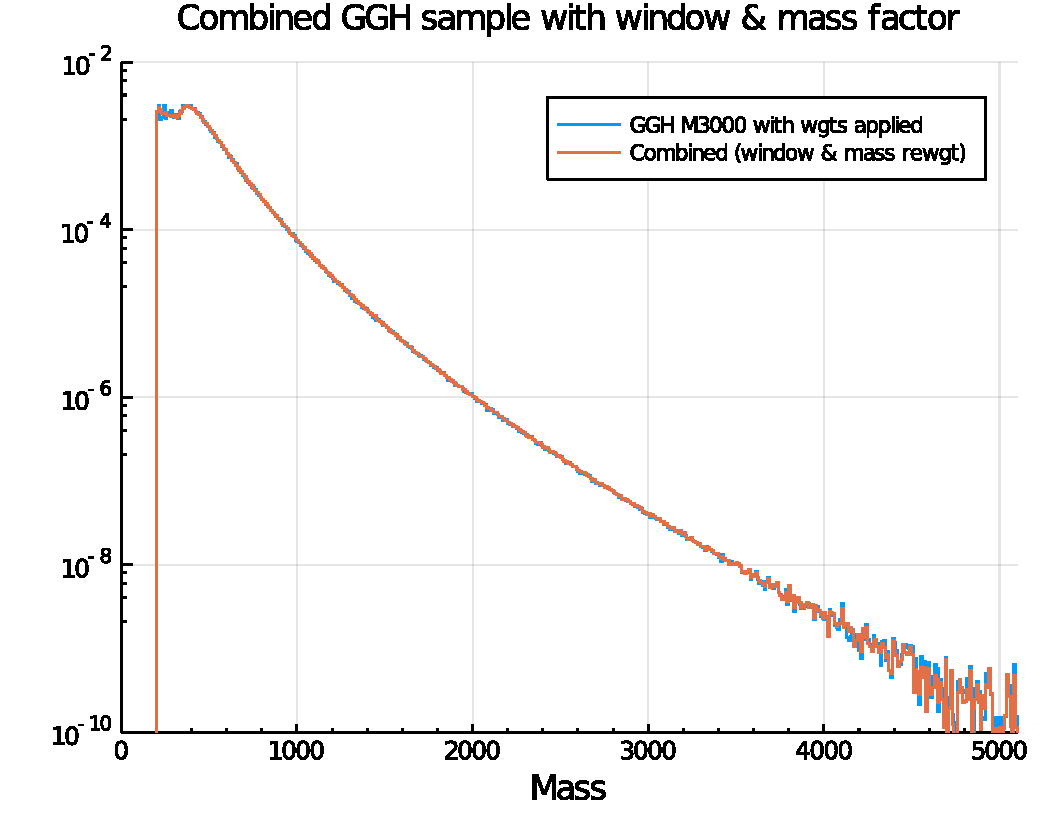
\includegraphics[width=.5\linewidth]{fig/LHC_compare_bothwgt.pdf}}
    \end{center}
    \caption{Iterative sample mass factors obtained (left) and the final combined sample (right)}
    \label{fig:LHE_rewgt}
\end{figure}

This factor corrects the high variations of overall normalizations between samples, the factors and result
are shown in Fig.~\ref{fig:LHE_rewgt}. As expected, high mass samples need a down correction (not by a lot)
to eliminate the deviated trend before. Complete tables of this weights for both samples can be found
in Appendix~\ref{apdx:mass_wgts}.

Finally, 1.10 is multiplied to the weights of all ggZZ processes (all of BKG, SIG, BSI
of GGH sample) as a K factor for Next-to-next-to-leading-order (NNLO) $\rightarrow$ 
Next-to-next-to-next-to-leading-order (N3LO) QCD.

Although we used the particular matrix element weights for one of the signal hypothesis, these two
correction factors apply to all hypothesis and a plot of them without unit area normalization are shown
in Fig.~\ref{fig:bsi_sig_bkg_compare}. As expected, background exceeds signal by more than 100\%
which is partially why the constrain is hard to obtain.
\begin{figure}[htb]
    \begin{center}
        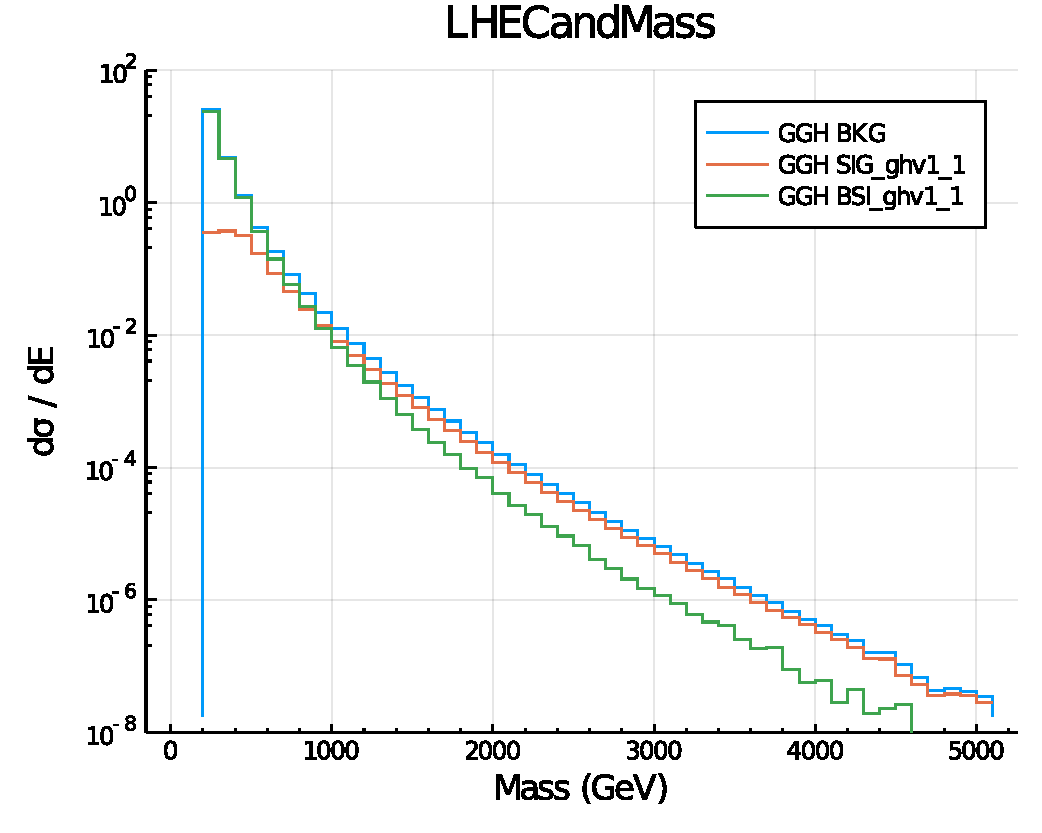
\includegraphics[width=.7\linewidth]{fig/LHE_integral_difference.pdf}
    \end{center}
    \caption{Distributions of background, signal, and background signal interaction}
    \label{fig:bsi_sig_bkg_compare}
\end{figure}

\section{Strategy in variable selection and binning and systematical uncertainties}
After preparing the signal samples and decided on the event selection criteria, we move on to
decide on the variables and their (2D histogram, as shown in Fig.~\ref{fig:templates_demo}) `binning' before a combined-limits
fit can be applied. As discussed in earlier sections, one of the more inventive variables
newly introduced specifically for the analysis is the DJJVBF discriminator. However, it is
clear that this variable is undefined for events with $\njets < 2$. To
not `waste' any statistical significance, we use $\met$ in its place for the
$\njets = 0,1$ categories. In total, we have 2 ($ee$ or $\mu\mu$) $\times$ 4 ($\njets = 0,1,2,3+$) = 8
channels to consider when making histogram templates.
Bin edges for different categories in number of jets are as the following:
\begin{itemize} 
    \item $\njets >= 2$
        \begin{itemize} 
            \item $\mtzz$ = 150, 300, 400, 600, 800, 1000, 13000 (GeV)
            \item KD1 = DJJVBF = 0, 0.2, 0.4, 0.6, 0.8, 1
        \end{itemize}
    \item $\njets < 2$
        \begin{itemize} 
            \item $\mtzz$ = 150, 300, 400, 600, 800, 1000, 13000 (GeV)
            \item KD1 = $\met$ = 125, 200, 280, 420, 500, 800, 13000 (GeV)
        \end{itemize}
\end{itemize}
The higher mass ($\mtzz$) bins are wider because samples
have difficulty filling them due to physical reasons (especially for backgrounds) 
and the cuts being applied. As shown in Fig.~\ref{fig:templates_demo}, the relative error (err/counts) of each
bin in the histogram templates are displayed, a balance between significance and uncertainty is
obtained. We use the above binning for all samples and 8 channels that are considered in this
thesis. See Appendix~\ref{apdx:templates_hist} for a compilation of template histograms of GGH sample.
\begin{figure}[hb]
    \begin{center}
        \subfloat[]{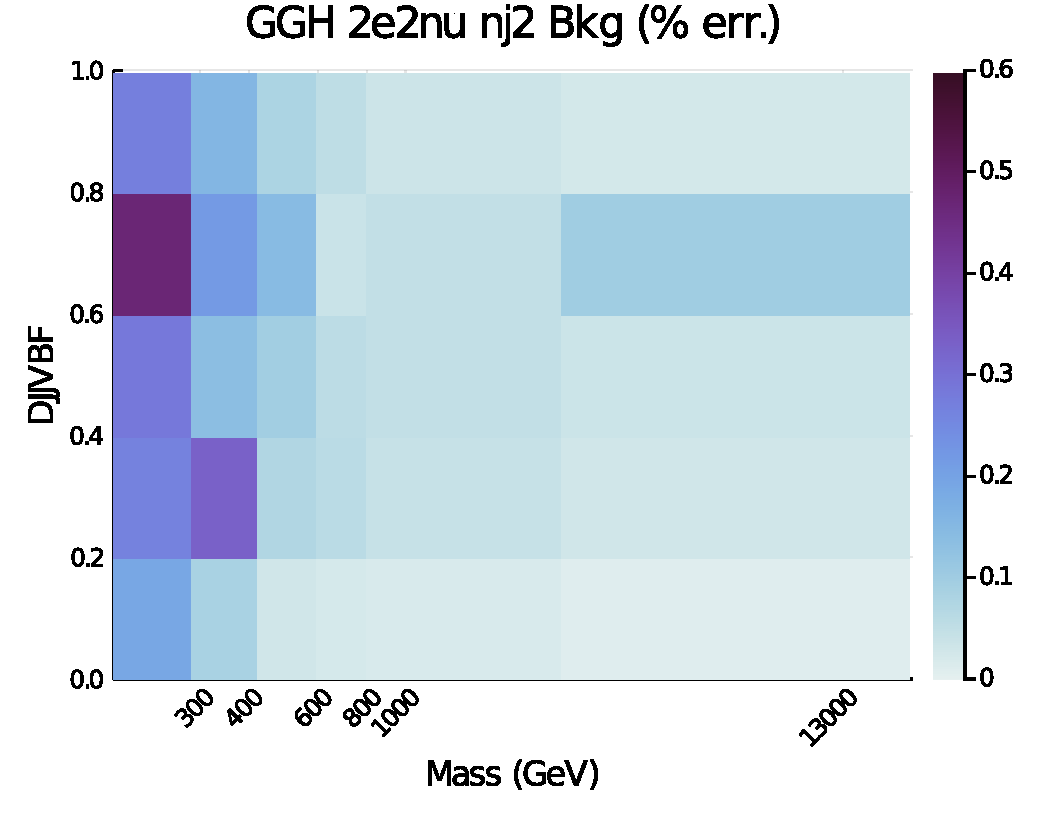
\includegraphics[width=.5\linewidth]{fig/ggZZ_templates/ggZZ_2e2nu_nj2_Bkg.pdf}}
        \subfloat[]{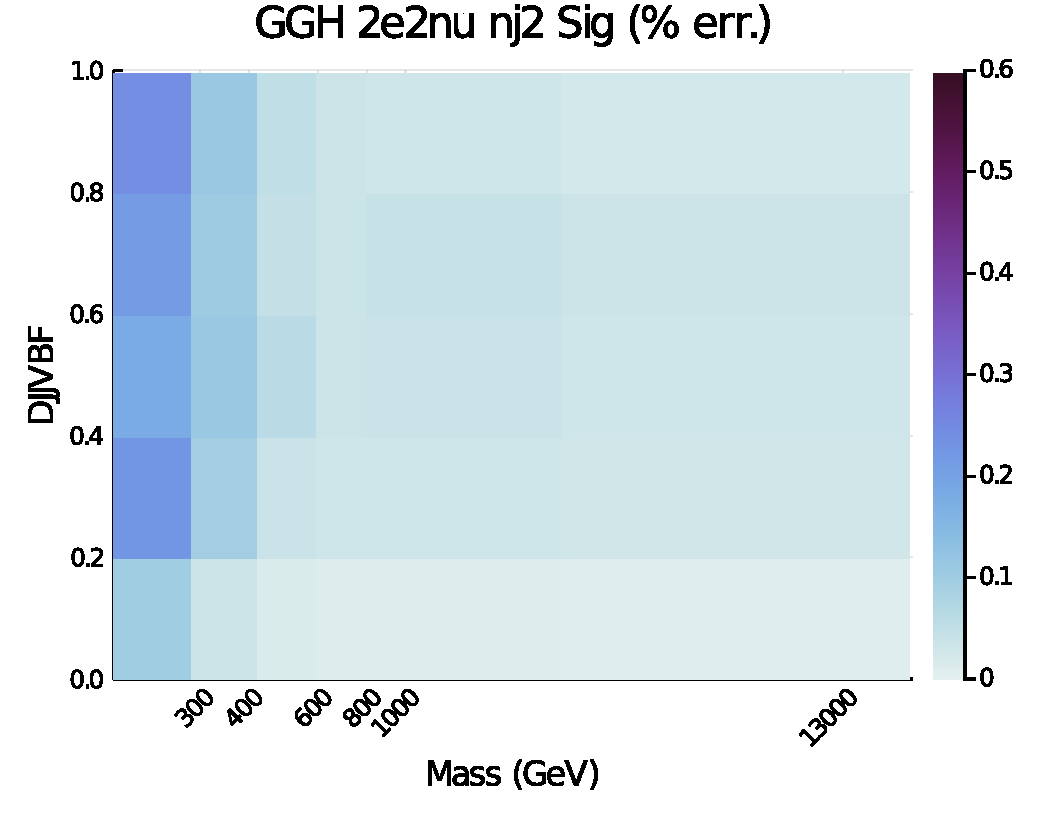
\includegraphics[width=.5\linewidth]{fig/ggZZ_templates/ggZZ_2e2nu_nj2_Sig.pdf}}
    \end{center}
    \caption{Background (left) and Signal (right) histogram templates for $2e2\nu$ with $\njets = 2$, showing
    percentage (statistical) error.}
    \label{fig:templates_demo}
\end{figure}

For low-yield background samples, due to the nature of NLO samples, bins sometimes would have negative
content. To mitigate it's effect on the likelihood fitting (pathological), we replace the bin content
by (Integral of the histogram) $\times \num{e-5}$.

Systematical uncertainties are also included in the fitting:
\begin{itemize}
    \item Luminosoties GGH\_ZZ, VBF\_ZZ, qqZZ, qqWZ
    \item NRB (non-resonant background) Estimation: TT, WW
    \item Branching Ratio of Higgs to ZZ to 4l: GGH\_ZZ, VBF\_ZZ
    \item K-fatcors of backgroun gluongluon parameter
\end{itemize}
See Table.~\ref{tab:uncertainty} for respective range of these uncertainties.
